%----------------------------------------------------------------------------------------
%	PACKAGES AND OTHER DOCUMENT CONFIGURATIONS
%----------------------------------------------------------------------------------------

\documentclass[twoside,twocolumn,9pt]{article}

\usepackage{blindtext} % Package to generate dummy text throughout this template 

%\usepackage[sc]{mathpazo} % Use the Palatino font
\usepackage{mathptmx}
\usepackage[T1]{fontenc} % Use 8-bit encoding that has 256 glyphs
\linespread{1.05} % Line spacing - Palatino needs more space between lines
\usepackage{microtype} % Slightly tweak font spacing for aesthetics

\usepackage{graphicx} 

\usepackage[english]{babel} % Language hyphenation and typographical rules

\usepackage[a4paper,left=0.71in,top=0.98in,right=0.71in,bottom=0.98in,columnsep=15pt]{geometry} % Document margins
\usepackage[hang, small,labelfont=bf,up,textfont=it,up]{caption} % Custom captions under/above floats in tables or figures
\usepackage{booktabs} % Horizontal rules in tables

\usepackage{enumitem} % Customized lists
\setlist[itemize]{noitemsep} % Make itemize lists more compact

\usepackage[runin]{abstract} % Allows abstract customization
\setlength{\abstitleskip}{-\parindent}
%\newcommand{\abstitlestyle}[1]{#1}
\renewcommand{\abstractnamefont}{\normalfont\bfseries\MakeUppercase} % Set the "Abstract" text to bold
\renewcommand{\abstracttextfont}{\normalfont} % Set the abstract itself to small italic text
\abslabeldelim{:}


\usepackage{titlesec} % Allows customization of titles
%\renewcommand\thesection{\Roman{section}} % Roman numerals for the sections
%\renewcommand\thesubsection{\roman{subsection}} % roman numerals for subsections
\titleformat{\section}[block]{\large\bfseries}{\thesection.}{1em}{} % Change the look of the section titles
\titleformat{\subsection}[block]{\large}{\thesubsection.}{1em}{} % Change the look of the section titles
\titleformat{\subsubsection}[block]{\normalsize}{\thesubsubsection.}{1em}{} % Change the look of the section titles

\usepackage{fancyhdr} % Headers and footers
\pagestyle{fancy} % All pages have headers and footers
\fancyhf{}% clear default for head and foot
\fancyhead[L]{
\includegraphics[scale=0.11]{figures/FISITA.png}}
\fancyhead[R]{\thepage}
\fancyfoot[L]{Proceedings of the FISITA 2020 World Congress, Prague, 14 - 18 September 2020}
\renewcommand{\headrulewidth}{0pt}
\fancypagestyle{firstpage}{
	\fancyhf{}% clear default for head and foot
	\renewcommand{\headrulewidth}{0pt}
	\pagestyle{fancy}
	\lhead{\textbf{F2020-VES-014}}
	\rhead{
\includegraphics[scale=0.15]{figures/FISITA.png}}
	\fancyfoot[L]{Proceedings of the FISITA 2020 World Congress, Prague, 14 - 18 September 2020}
}
\usepackage{xpatch}
\xapptocmd{\titlepage}{\thispagestyle{firstpage}}{}{}

\usepackage{titling} % Customizing the title section

%\usepackage{hyperref} % For hyperlinks in the PDF

\usepackage{authblk}

\usepackage{caption}
\DeclareCaptionLabelFormat{nospace}{#1#2}
\captionsetup[table]{labelfont=normal, textfont=normal,name=Table ,labelsep=period, justification=raggedright, singlelinecheck=off}
\captionsetup[figure]{labelfont=normal, textfont=normal,name=Figure ,labelsep=period, justification=raggedright, singlelinecheck=off}
\usepackage[utf8]{inputenc}   				 	%% utf8 support (required for biblatex)
\usepackage{silence}  							%% For filtering warnings
\usepackage[style=ieee,doi=false,isbn=false,url=false,date=year,backend=biber,maxbibnames=15,maxcitenames=2,mincitenames=1,uniquelist=false,uniquename=false,giveninits=true]{biblatex}
% Filter warnings issued by package biblatex starting with "Patching footnotes failed"
\WarningFilter{biblatex}{Patching footnotes failed}
%\renewcommand*{\bibfont}{\footnotesize}		%% Use this for papers
\renewcommand*{\bibfont}{\small}
\setlength{\biblabelsep}{\labelsep}
\bibliography{../bib}
\usepackage[fleqn]{amsmath}

\usepackage{xcolor}
\usepackage[capitalize]{cleveref}
\crefname{figure}{Figure}{Figures}

% Table stuff
\usepackage{booktabs}
\usepackage{tabularx}
\setlength{\heavyrulewidth}{0.1em}
\newcommand{\otoprule}{\midrule[\heavyrulewidth]}

\usepackage{xcolor}
\usepackage{tikz}
\usepackage{pifont} % \ding{}
\definecolor{resultfail}{rgb}{1.,0,0}
\definecolor{resultacceptable}{rgb}{1,0.76.,0}
\definecolor{resultfair}{rgb}{0,0.69.,0.94}
\definecolor{resultgood}{rgb}{0,0.69.,0.31}
\newcommand{\mycircle}[2]{\tikz \path[draw=#1, fill=#2] (0, 0) circle (1ex);}
\newcommand{\mysquare}[2]{\tikz \path[draw=#1, fill=#2] (0, 0) rectangle (2ex, 2ex);}
\newcommand{\fail}{\mycircle{resultfail}{resultfail}}
\newcommand{\acceptable}{\mycircle{resultacceptable}{resultacceptable}}
\newcommand{\fair}{\mycircle{resultfair}{resultfair}}
\newcommand{\good}{\mycircle{resultgood}{resultgood}}
\newcommand{\pass}{\textcolor{green}{\ding{52}}}
\newcommand{\nopass}{\textcolor{red}{\ding{55}}}
\newcommand{\nonconformity}{\mysquare{black}{yellow}}
\newcommand{\observation}{\mysquare{black}{blue}}




%----------------------------------------------------------------------------------------
%	TITLE SECTION
%----------------------------------------------------------------------------------------

\providecommand{\keywords}[1]{\textbf{KEY WORDS:} #1}

\pretitle{\begin{center}\huge\normalfont\MakeUppercase} % Article title formatting
\posttitle{\end{center}\vskip 1em} % Article title closing formatting
\title{type the title of the paper here} % Article title

\author[1,2]{\large\bfseries Erwin de Gelder}
\author[1]{\large\bfseries Olaf Op den Camp}
%\author[1,3]{\large\bfseries Jan-Pieter Paardekooper}
%\author[2]{\large\bfseries Bart De Schutter}

\affil[1]{\normalsize\textit{TNO, Integrated Vehicle Safety, Helmond, The Netherlands (E-mail: erwin.degelder@tno.nl, olaf.opdencamp@tno.nl)}}
\affil[2]{\normalsize\textit{Delft University of Technology, Delft Center for Systems and Control, Delft, The Netherlands}}
%\affil[3]{\normalsize\textit{Radboud University, Donders Institute for Brain, Cognition and Behaviour, Nijmegen, The Netherlands}}
\date{} % Leave empty to omit a date

\renewcommand{\maketitlehookd}{%
\begin{abstract}	
\noindent The development of Autonomous Vehicles (AVs) has made significant progress in the last years and it is expected that AVs will soon be introduced on our roads. An important aspect in the development of AVs is the assessment of their safety. As traditional methods for safety assessment of vehicles are not feasible to be performed for AVs within reasonable time and cost, new approaches need to be worked out. Among these, real-world scenario-based assessment is widely supported by many players in the automotive field. Scenario-based assessment allows for using virtual simulation tools in addition to physical tests, such as on a test track, proving ground, or public road.

We propose a procedure for real-world scenario-based road-approval assessment considering three stakeholders: the applicant, the assessor, and the (road or vehicle) authority. In this procedure, the applicant applies for the approval of one specific AV, the assessor assesses this AV and advises the authority, and the authority sets the requirements for the AV and decides whether this specific AV is approved for road testing The challenges are as follows. Firstly, the tests need to be tailored to the operational design domain (ODD) and dynamic driving task (DDT) description of the AV. Secondly, it is assumed that the applicant does not want to disclose all of the detailed test results because of proprietary or confidential information contained in these results. Thirdly, due to the complex ODD and DDT, many test scenarios are required to obtain sufficient confidence in the assessment of the AV. Consequently, it is assumed that due to limited resources, it is infeasible for the assessor to conduct all (physical) tests. 

We propose a systematic approach for determining the tests that are based on the requirements set by the authority and the AV’s ODD and DDT description, such that the tests are tailored to the applicable ODD and DDT. Each test comes with metrics that enables the applicant to provide a performance rating of the AV for each of the tests. By only providing a performance rating for each test, the applicant does not need to disclose the details of the test results. In our proposed procedure, the assessor only conducts a limited number of tests. The main purpose of these tests is to verify the fidelity of the results provided by the applicant. Still, the applicant needs to conduct many tests, but this is assumed to be feasible because the applicant can utilize virtual simulation tools to conduct (a part of) the tests whereas this is not possible for the assessor due to proprietary or confidential information. To illustrate the proposed procedure, an example is presented.

\keywords{safety assessment, autonomous vehicle, scenario-based assessment}
\end{abstract}
}

%----------------------------------------------------------------------------------------

\begin{document}
	
% Print the title
\maketitle
\thispagestyle{firstpage}
%----------------------------------------------------------------------------------------
%	ARTICLE CONTENTS
%----------------------------------------------------------------------------------------

\section{Introduction}
\label{sec:introduction}

TODO

\color{red}
For Arash and Hala: please use \\{\tt \textbackslash cref\{sec:introduction\}}\\ to refer to sections, figures etc. It automatically adds things as `Section': e.g., \cref{sec:introduction}.
\color{black}

The introduction contains: 
\begin{itemize}
	\item Setting up the context of automated driving
	\item Giving some background information about the hazard analysis and risk assessment in the ISO~26262 standard
	\item The gap (the problem) We currently have this as a separate chapter, we could move it to introduction depending on the length. 
	\item our contribution. 
	\item paper structure
\end{itemize}
\section{Problem definitions}
\label{sec:problem} % Arash

This Section presents: 
\begin{itemize}
	\item Why risk assessment matters?
	\item What is currently the risk estimation method? 
	\item What is lacking in this approach? 
	\item What need to be done more? 
\end{itemize}

In this section we position our research in the automotive safety engineering domain. 
We present the current risk assessment methods and discuss their limitation and the impact of these limits.
The argue that advancement in the risk assessment methods are required for achieving higher levels of automation in the automotive domain. 

\subsection{Why risk assessment?}

Safety means avoiding risk. 
The risk associated with driving may come from multiple sources. 
It could be a traffic situation in which a sequence of uncorrelated actions performed by different actors lead to an accident. 
The risk could also be due to technical failure originating from a system fault. 
%This type of faults and failures should be avoided by the manufacturers of the automotive systems (OEMs and Tiers), 
%	while the later is a responsibility of the traffic participants. 
For the former, the manufacturers are deemed responsible; 
	therefore, they put a lot of effort on the quality  assurance of their products 
		and for understanding and mitigating technical safety issues.  
The later comes into the public domain and road authorities are responsible for minimizing the risk by good design of roads and traffic rules. 
The  risk, however, cannot be avoided fully. 
There is always a certain amount of \textit{residual risk} remaining after taking risk avoidance/mitigation measures. 

Understanding the risk and measuring it is crucial in both directing the effort on avoiding or mitigating the impacts. 
Moreover, formulating and opinion about when using a system is ``safe enough'' depends on the ability to measure the risk. 
	

\subsection{Risk assessment in ISO~26262}

Risk is defined in ISO~26262 as:
\begin{definition}
	``combination of the probability of occurrence of harm and the severity of that harm'' 
\end{definition}



Risk assessment is an integral part of the safety life-cycle of ISO~26262 and one of the earlier activities. 
During risk assessment, the identified hazardous events are analyzed and the associated severity, probability of exposure and controllability are estimated and assigned to some predefined levels. 
The combination of the estimated severity, exposure and controllability contribute to construct the Automotive Safety Integrity Level (ASIL). 


This is the domain of functional safety. 
The goal of functional safety is to avoid \emph{unreasonable} risk\footnote{Unreasonable risk is judged according to the the society's acceptance of level of risk.} that is due to some sort of malfunctioning.


\section{Procedure for the safety assessment}
\label{sec:procedure}

This paper assumes that many of the relevant tests for the safety assessment are performed in a virtual simulation environment that is controlled by the applicant. The proposed procedure intends to consider all results, both from virtual simulation and from actually performed physical tests. Where the assessor does not have access to the required models of the AV under test, the assessor will have the capability to perform physical tests on the AV. How to balance between the different results in the assessment, considering virtual and physical test results of the applicant and physical test results of the assessor is schematically presented in \cref{fig:procedure}. Each rectangular block represents an action. The procedure distinguishes between actions for which the applicant is responsible and actions for which the assessor is responsible. The procedure consists of the following actions:
\begin{enumerate}
	\item The first action is to derive which system-level tests need to be performed with reference to the ODD and DDT of the AV under test. Here, “system-level” is mentioned explicitly, because it is assumed that also in case of a failure of any of the subsystems, the AV would fail the system-level tests. Note, however, that it is advised that the applicant ensures that each of the subsystems underwent a rigorous assessment before applying for the AV assessment. 
	\item If the derived tests are acceptable, the next action is to select the tests for the assessment. Here, a distinction is made between tests for which the applicant is fully responsible and physical tests that are conducted by the assessor. The latter will focus more on spot checking.
	\item Once the tests are selected, these tests need to be conducted. The results of these tests will be described using prescribed metrics. Note, however, that these metrics may not contain too much information as it is assumed that the applicant does not want to disclose details of sensor and system implementation or even detailed test results because of the proprietary or confidential information contained in these results. 
	\item The final step is to assess the results from the tests and to formulate an advice for the authority on whether the AV is ready for deployment and under which conditions.
\end{enumerate}

\begin{figure*}
	\centering
	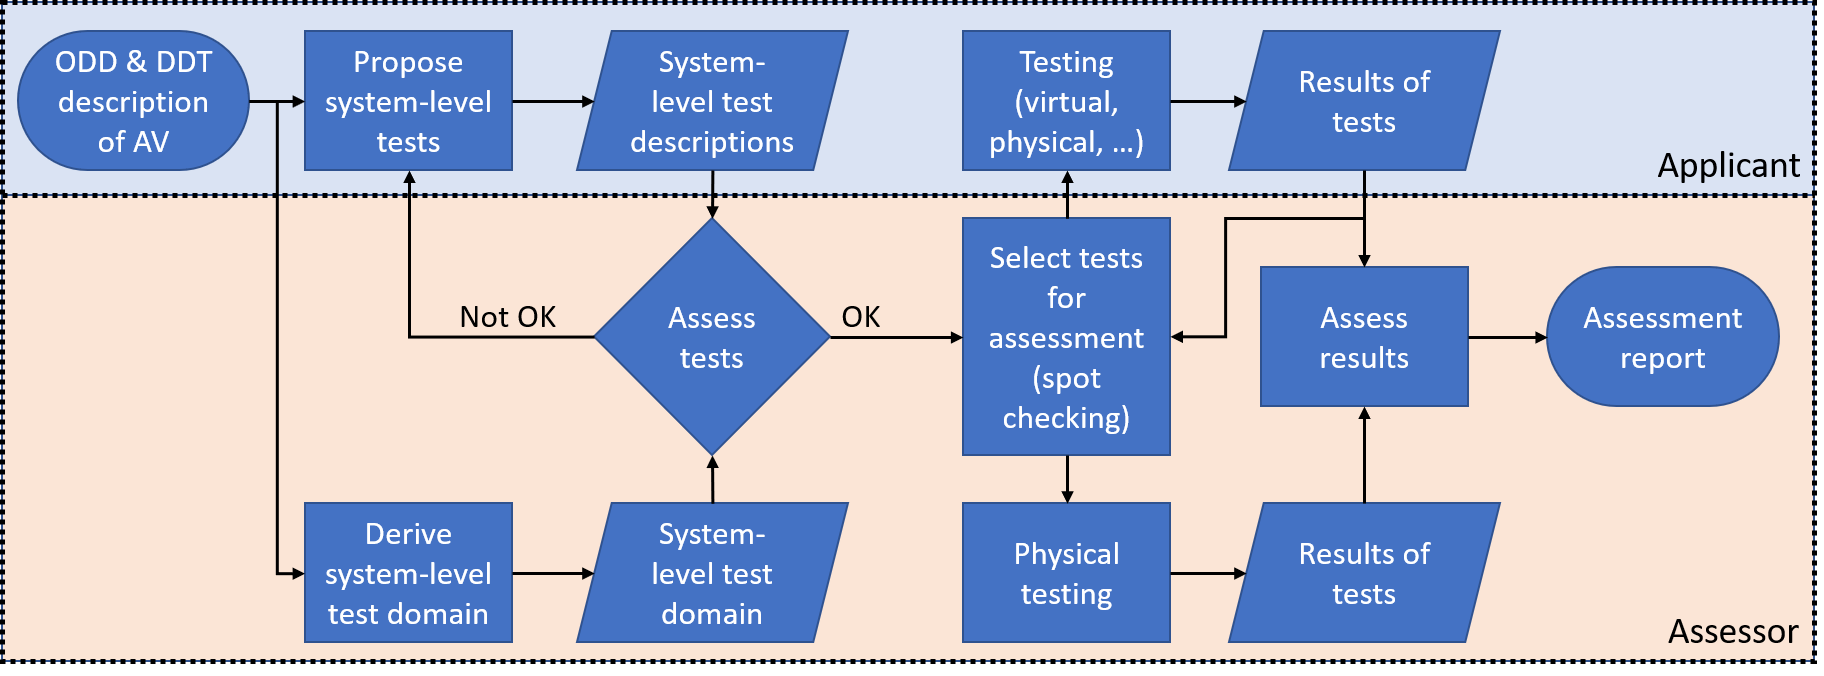
\includegraphics[width=\linewidth]{figures/procedure}
	\caption{Proposed framework for the safety assessment of an autonomous vehicle (AV).}
	\label{fig:procedure}
\end{figure*}

In the following sections, each of the actions are further detailed. We end this section with a short note on monitored deployment in case of a successful completion of the assessment.



\subsection{Deriving test descriptions}
\label{sec:test descriptions}

Based on the ODD and the DDT of the AV, the tests are derived. Following the same reasoning as \textcite{stellet2015taxonomy}, a test is an evaluation of:
\begin{itemize}
	\item a statement on the system-under-test (test criteria; what are we going to evaluate using the test);
	\item under a set of specified conditions (test case; how are we going to evaluate the test criteria);
	\item using quantitative measures (metrics; how to express the outcome of the test quantitatively);
	\item and a reference of what would be the acceptable outcome (reference; when is the outcome acceptable).
\end{itemize}

Since the applicant has designed and developed the AV, it is expected that the applicant has a clear notion of the tests that are required for a complete assessment of the AV and which the AV should appropriately handle. Similarly, if the set of relevant test descriptions is not complete during the development of the AV, it is conceivable that the AV will not operate safely for all circumstances possible within the ODD. 

Although it is expected that the applicant provides all relevant test descriptions, it is important that the applicant and the assessor discuss these test descriptions, and that a check is made whether or not the test descriptions are complete and cover the ODD sufficiently. If an important test description is missing, it is conceivable that the AV is not specifically designed to pass the corresponding test. In order to assess the completeness of the test descriptions provided by the applicant, the assessor needs to define the test domain for the relevant system-level test descriptions and use these to investigate if any important test descriptions are missing. Here, the so-called test domain refers to a more high-level description of the range of tests that are expected, rather than an enumeration of the large number of relevant tests.

If it turns out that the test descriptions that are provided by the applicant are not complete, the process needs to be restarted, as indicated by the ``Not OK'' line in \cref{fig:procedure}. On the other hand, if the test descriptions are deemed to be complete enough, the assessment proceeds to the next step: selecting tests for the assessment.



\subsection{Selecting tests for the assessment}
\label{sec:selection}

In principle, the applicant is expected to provide results for all tests. In the next section, we explain how these results may look like. Based on these results, tests are selected for the physical testing performed by the assessor. This is indicated by the arrow pointing from ``results of tests'' of the applicant to ``select tests for assessment'' in \cref{fig:procedure}.  

A test is selected for physical testing by the assessor if any of the following three statements are true:
\begin{itemize}
	\item The applicant does not provide a result. Although the applicant is expected to provide results for most tests, it might be possible that there are some tests for which the applicant does not have the resources to perform the tests reliably, for example if specific tooling is required. Note, however, that if the applicant does not provide results for too many tests, the assessment automatically results in a fail.
	\item The result seems inconsistent. If there is sufficient reason for the assessor to not confide in the result provided by the applicant, the test can be performed by the assessor to check the result provided by the applicant.
	\item The test is selected for spot checking. The main reason to perform spot checking is to assess the fidelity of the results provided by the assessor.
\end{itemize}
The process of test selection is summarized in \cref{fig:selection}.

\begin{figure}
	\centering
	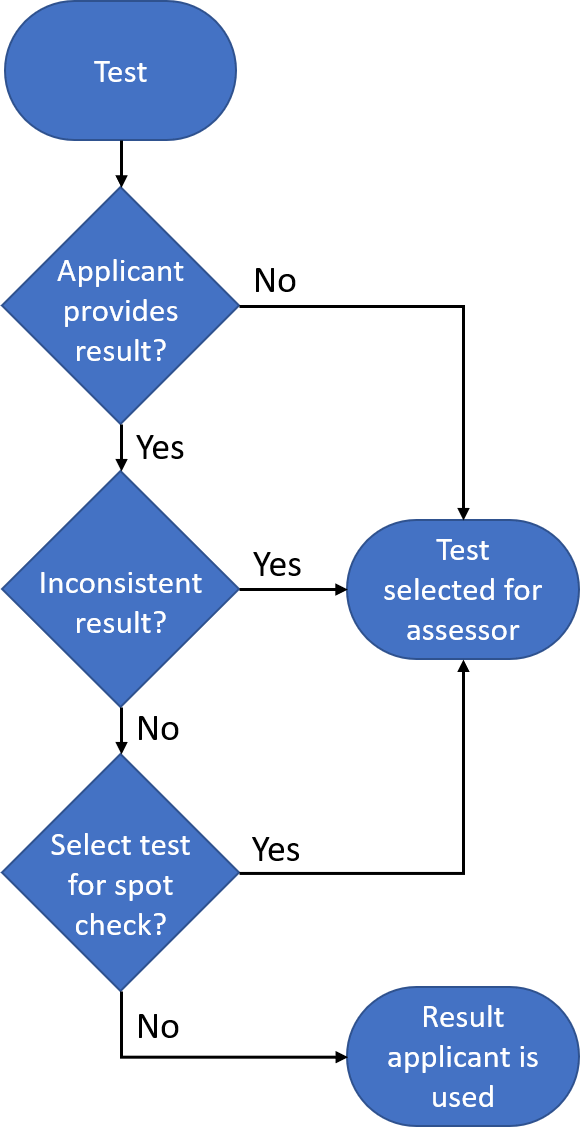
\includegraphics[width=.65\linewidth]{figures/test_selection}
	\caption{Decision scheme for the selection of a test for physical assessment by the assessor.}
	\label{fig:selection}
\end{figure}



\subsection{Testing}
\label{sec:testing}

As explained in the previous section, the applicant is expected to provide results for most tests. However, it is assumed that the applicant does not want to disclose detailed test results. Therefore, a rating scheme is proposed. Using a specific metric for each test, three references are defined: an acceptable result, a fair result, and a good result. If the result of the test is worse that the acceptable result, a ``fail'' is reported. If the result passes the acceptable reference but not the what is defined as a fair result, an ``acceptable'' is reported. Similarly, a ``fair'' is reported if the result is between a fair and a good result. If the result is better than what has been defined as a good result, a ``good'' is reported. This is schematically shown in \cref{fig:rating}. 

\begin{figure}
	\centering
	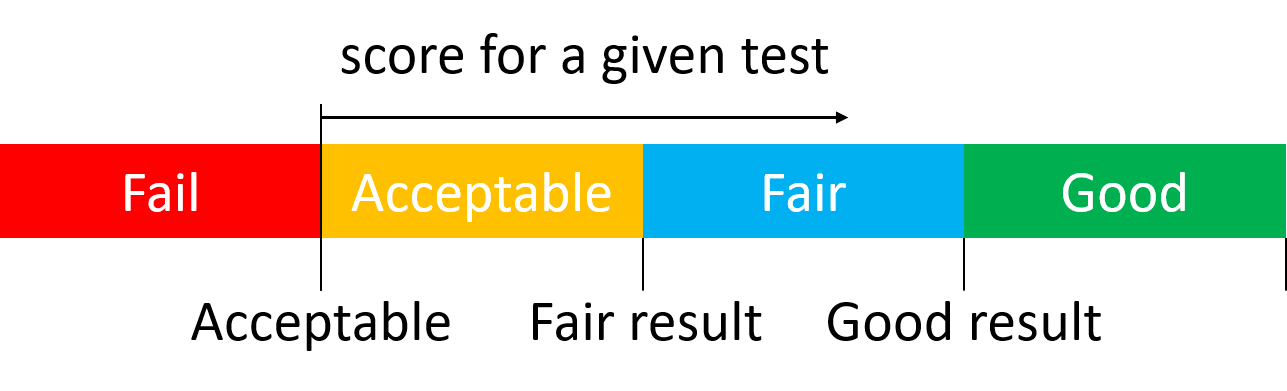
\includegraphics[width=\linewidth]{figures/rating}
	\caption{Different scoring options per test.}
	\label{fig:rating}
\end{figure}

In principle, the applicant is free to choose any method to derive the results. However, considering the large number of tests, the use of virtual simulations seems inevitable. In practice, it is expected that a both virtual simulations, physical tests, and a combination, such as hardware-in-the-loop testing, is used to determine the test results.

On the other hand, the tests by the assessor are performed physically. The main reason for this is that virtual simulations are ruled out as that would require the applicant to provide a model of the AV, which is expected to be impossible because of proprietary reasons.



\subsection{Assess results}
\label{sec:assess results}

The following assessment results are distinguished per test:
\begin{itemize}
	\item In case the test results show that for the specific test the AV performs acceptable (i.e., ``acceptable'', ``fair'', or ``good'', see \cref{fig:rating}), the test is passed. If this is not the case, then the specific test fails.
	\item Inspired by ISO~9001 on quality management \autocite{ISO9001}, a passed test may result in a non-conformity. An “acceptable” result automatically leads to a non-conformity (NC). This means that the response of the AV deviates substantially from  response that is qualified as “good”, but the deviation is not severe. Since the AV meets the minimum requirement for this test and consequently safety is not compromised, there is no reason to fail the AV based on this test. Nevertheless, an NC is issued to indicate that the applicant is asked to consider improvements, e.g., for a next version of the system.
	\item In case the test is also performed by the assessor and the corresponding result is worse than the reported result of the applicant, this also leads to a NC.
	\item The assessment of a test result might come with an observation (OB) that needs consideration of the applicant. 
\end{itemize}

If a test results in a fail, then either the assessment results in a negative advice of the assessor to the authority or it is advised to only allow for deployment of the AV under certain conditions. For example, if the only tests that are failed consider low-light conditions, the AV might be deployed under the condition that it operates only from sunrise till sunset. 

NCs and OBs do not lead to an immediate fail of the assessment. However, it is likely that they lead to a fail in a future assessment, e.g., when test criteria become increasingly demanding, and the applicant does not appropriately consider such NCs or OBs. NCs provide information to the applicant on how requirements might develop in the future, which, consequently, gives direction and motivation on continuous improvement of AVs regarding safety. On the other hand, many NCs – the AV barely passes the test in many cases – might mean that safety is compromised and, therefore, it might also result in a negative advice of the assessor to the authority regarding the deployment of the AV.

Note that when many NCs are observed, the AV probably will not be able to pass all tests if all tests would be performed physically by the assessor. Theoretically, this is however still possible. To minimize the risk of having an AV that passes all tests, but with many NCs, a system using demerit points is introduced. The AV starts with, e.g., 100 points, and in the assessment, 1, 2, or 3 points are subtracted for each NC, depending on the severity of the NC. Once the number of points for the AV are reduced to 0, then the AV is indicated to have failed he assessment because of an overrun of NCs. The numbers given here are merely provided as an example.



\subsection{Monitored deployment}
\label{sec:monitored deployment}

A successful completion of the proposed assessment might result in the approval for the deployment of the AV under the condition that the behavior of the AV on the road is continuously monitored. We propose that during such a deployment phase, the applicant is required to upload detailed driving data to allow for monitoring the AV behavior. This is implemented for two reasons:
\begin{itemize}
	\item After completion of the assessment pipeline, road and/or vehicle authorities may require the monitoring of safety continuously when driving on the public road.
	\item The uploaded data may be used to improve the generation of tests and the selection of relevant test cases for a particular AV, as is possible that some tests have been overlooked during the initial assessment process or that situations on the road gradually change with changes in traffic, e.g.because of the introduction of new mobility systems.
\end{itemize}

The feedback to the data acquisition element allows for ongoing learning and improvement of the standards and assessment systems, while being able to adapt to new types of transportation such as personal mobility devices. For example, additional test cases could be identified and incorporated into future safety assessment procedures. A deployment might consider new operational areas, the extension of the scenario database with scenarios that potentially differ between such areas would then be covered. Moreover, to obtain a scenario database that is `complete', i.e., statistically accurate, it is expected that operational data collection is required over an extended period, which most probably will not be realized before the deployment is operationalized. In other words, the imperfection of the assessment framework should not become a barrier for the introduction of new safe mobility solutions onto the market, in case these devices are tested to be safe for all currently known conditions. The assessment method, especially the step regarding monitored deployment, supports the continuous increase in knowledge on the state-of-the-art of road safety and herewith prepares the safety assessment method to be sustainable for the future.

\section{Case Study} % Erwin & Hala
%\label{sec:example}

In this section, we present a case study to illustrate the method of quantifying the risk for a cut-in scenario. We will first describe the cut-in scenario and the use case. The actual system for which the risk is computed is presented in next. After these two steps, we will go through the steps of our proposed method.



\subsection{The cut-in scenario and the use case}
%\label{sec:scenario class}

We want to quantify the risk for cut-in scenarios that are linguistically described as follows: while the ego vehicle drives at a moderate to high speed while staying in its lane, another vehicle cuts into the lane of the ego vehicle, such that this vehicle becomes the ego vehicle's lead vehicle. Furthermore, the ego vehicle needs to brake to prevent a collision.

For the quantification of the risk, 60 hours of data (see also \cite{deGelder2017assessment}) are collected by driving a specific route in and between Eindhoven and Helmond, The Netherlands, with twenty different drivers, each driving the route twice. Therefore, it is assumed that the use case of the AD system is driving this route. We will use the data for the estimation of the risk. Hence, we will make use of the following assumption:
\begin{assumption}
	The recorded naturalistic driving data is representative for what a vehicle with the AD system might encounter along the same route.
\end{assumption}



\subsection{System-under-test}
%\label{sec:system}

To reduce efforts for the assessment, often simulations are employed. However, even simulations can consume considerable time, as these simulations might run real-time \cite{shah2018airsim} or slower when a higher level of detail is used \cite{zofka2016testing}. For our method, we will simplify the simulations, such that the total required time on a common computer is in the order of minutes. Since we are interested in approximate results, a high level of detail is not required. 

To simplify the system-under-test, it is assumed that the system's desired acceleration is similar to the adaptive cruise control defined in \cite{deGelder2017assessment}, i.e.,
\begin{equation}
	\label{eq:desired acceleration} 
	u(t) = k_{\mathrm{d}}(v(t))(d(t) - \tau_{\mathrm{h}} v(t) - s_0) + k_{\mathrm{v}}\left(\dot{d}(t) - ha(t) \right),
\end{equation}
with
\begin{equation}
	\label{eq:gain}
	k_{\mathrm{d}}(v(t)) = k_{\mathrm{d1}} + \left( k_{\mathrm{d2}} - k_{\mathrm{d1}} \right) \exp \left\{ -\frac{v(t)^2}{2\sigma_{\mathrm{d}}} \right\}.
\end{equation}
Here, $v$ is the speed of the ego vehicle, $d$ denotes the clearance between the ego vehicle and its predecessor, i.e., the vehicle that performs the cut-in. The relative speed is denoted by $\dot{d}$ and $a$ refers to the acceleration of the ego vehicle. The ego vehicle is modeled using a first order model with a time delay, i.e.,
\begin{equation}
	\label{eq:vehicle model}
	\tau \dot{a}(t) + a(t) = u(t - \theta).
\end{equation}
Furthermore, the deceleration is limited at $\unit[-6]{ms^{-2}}$. A description of the constants of \cref{eq:desired acceleration,eq:gain,eq:vehicle model} are listed in \cref{tab:constants}. The controller runs at \unit[100]{Hz}.

\begin{table}
	\centering
	\caption{The constants used for the simple automation system of \cref{eq:desired acceleration,eq:gain,eq:vehicle model}.}
	\label{tab:constants}
	\begin{tabular}{clc}
		\toprule
		Parameter & Description & Value \\ \otoprule
		$\tau_{\mathrm{h}}$ & Desired headway time & \unit[2.0]{s} \\
		$s_0$ & Safety distance & \unit[1.5]{m} \\
		$k_{\mathrm{d1}}$ & Distance gain at high speed & $\unit[0.7]{s^{-2}}$ \\
		$k_{\mathrm{d2}}$ & Distance gain at low speed & $\unit[2.0]{s^{-2}}$ \\
		$\sigma_{\mathrm{d}}$ & Shaping coefficient of distance gain & $\unit[5]{ms^{-1}}$ \\
		$k_{\mathrm{v}}$ & Speed difference gain & $\unit[0.35]{s^{-1}}$ \\
		$\tau$ & Time constant of the vehicle model & \unit[0.1]{s} \\
		$\theta$ & Delay of the vehicle response & \unit[0.2]{s} \\
		\bottomrule
	\end{tabular}
\end{table}

Note that there is no intervention of a human:
\begin{assumption}
	The ego vehicle is fully controlled by the automation system as defined by \cref{eq:desired acceleration,eq:gain}. Hence, there is no intervention of a human.
\end{assumption}



\subsection{Calculate exposure}
%\label{sec:example exposure}

The cut-in scenarios are subject to the following conditions:
\begin{itemize}
	\item $C_1$: The speed of the ego vehicle is within the range of \unit[60]{km/h} and \unit[130]{km/h}.
	\item $C_2$: There are no restrictions on the weather conditions.
	\item $C_3$: There are no restrictions on the lighting conditions.
\end{itemize}

Obviously, because there are no restrictions to the weather and lighting conditions, we have $P(C_2,C_3)=1$. For the first condition, we can use the data to estimate the likelihood. The data, however, has been recorded during sunny weather at daylight. Therefore, we need to following assumption.

\begin{assumption} \label{asm:conditions}
	Let $C_2'$ and $C_3'$ denote the conditions of having sunny weather and daylight, respectively. Then we have $P(C_1|C_2,C_3)=P(C_1|C_2',C_3')$.
\end{assumption}

From the data, it appeared that $P(C_1|C_2',C_3')=0.20$. Using \cref{asm:conditions}, we have
\begin{equation}
	P(C) = P(C_1,C_2,C_3) = P(C_1|C_2',C_3')\cdot P(C_2,C_3) = 0.20.
\end{equation}

The cut-in scenarios consist of the following activities:
\begin{itemize}
	\item $A_1$: The ego vehicle is lane following.
	\item $A_2$: The target vehicle is driving in an adjacent lane in the same direction as the ego vehicle.
	\item $A_3$: After activity $A_2$, the target vehicle performs a lane change towards the lane of the ego vehicle, such that the ego vehicle needs to brake.
	\item $A_4$: The automation system detects the cut-in.
	\item $A_5$: After activity $A_4$, the automation system activates the brakes of the ego vehicle.
\end{itemize}

The likelihood of the activities $A_1$, $A_2$, and $A_3$ can be estimated using the data. It is assumed that the ego vehicle needs to brake if the target vehicle is driving slower and the headway time is less than three seconds. In case of a slower target vehicle with a larger headway time, the scenario is referred to as a gap closing scenario \cite{semsarkazerooni2016cacc, gelder2016pacc}.

For simplicity, we assume the following:
\begin{assumption}
	The automation system always detects the cut-in and activates the brakes after detecting the cut-in, such that $P(A_4,A_5|A_1,A_2,A_3,C) = 1$.
\end{assumption}

Using this assumption, we can compute $\lambda_{A|C}$ by detecting the number of occurrences of the activities $A_1$, $A_2$, and $A_3$ under the conditions $C$. Based on the dataset, we have $\lambda_{A|C}=\unit[9.9]{h^{-1}}$, i.e., in each hour that the ego vehicle is driving in a speed range of \unit[60]{km/h} and \unit[130]{km/h}, there are on average $9.9$ cut-ins with the target vehicle driving slower than the ego vehicle, such that the headway time after the cut-in is less than three seconds. From this, it simply follows that
\begin{equation}
	\lambda_{A,C} = \lambda_{A|C} \cdot P(C) = 2.0.
\end{equation}



\subsection{Calculating severity}
%\label{sec:example severity}

To limit the number of parameters, we assume the following:
\begin{assumption}
	The ego vehicle is driving at a constant speed at the moment of the cut-in of the target vehicle, i.e., the moment that the target vehicle enters the lane of the ego vehicle.
\end{assumption}
\begin{assumption}
	The target vehicle is driving at a constant speed.
\end{assumption}
Both assumptions can be justified using the data. In case of the ego vehicle, the average acceleration at the moment of the cut-in is $\unit[-0.29]{ms^{-2}}$ and the standard deviation equals $\unit[0.50]{ms^{-2}}$. In case of the target vehicle, the average deceleration at the moment of the cut-in is $\unit[0.05]{ms^{-2}}$ and the standard deviation equals $\unit[0.37]{ms^{-2}}$. As a result, the scenario is parametrized using $d=3$ parameters:
\begin{enumerate}
	\item The clearance between the target vehicle and the ego vehicle at the moment of the cut-in, i.e., the moment than the target vehicle enters the lane of the ego vehicle.
	\item The speed of the ego vehicle at the moment of the cut-in.
	\item The speed of the target vehicle throughout the whole scenario.
\end{enumerate}


A histogram of the data of the parameters is shown in \cref{fig:histogram}. The probability density function is estimated using the KDE of \cref{eq:kde} with the Gaussian kernel of \cref{eq:gaussian kernel}. Before applying KDE, the data is scaled, such that the standard deviation equals one for each parameter. We use leave-one-out cross validation to compute the bandwidth $h$ (see also \cite{duin1976parzen}) because this minimizes the Kullback-Leibler divergence between the real underlying pdf and the estimated pdf \cite{turlach1993bandwidthselection,zambom2013review}. The resulting bandwidth equals $h=0.198$. The marginal probability distributions coming from the resulting joint distribution, i.e. the KDE, are shown in \cref{fig:histogram} by the black lines.

\setlength\figurewidth{0.5\linewidth}
\setlength\figureheight{0.25\linewidth}
\begin{figure}
	\centering
	% This file was created by matplotlib2tikz v0.6.17.
\begin{tikzpicture}

\begin{groupplot}[group style={group size=1 by 3}]
\nextgroupplot[
xlabel={Clearance [m]},
ylabel={Density},
xmin=8.12085897227673, xmax=100.239482786353,
ymin=0, ymax=0.0358233749416452,
width=\figurewidth,
height=\figureheight,
tick align=outside,
tick pos=left,
x grid style={white!69.01960784313725!black},
y grid style={white!69.01960784313725!black},
axis x line*=bottom,
axis y line*=left,
scaled y ticks = false,
y tick label style={/pgf/number format/fixed}
]
\draw[draw=black,fill=gray] (axis cs:12.3080691456438,0) rectangle (axis cs:16.4952793190109,0.0120414705686202);
\draw[draw=black,fill=gray] (axis cs:16.4952793190109,0) rectangle (axis cs:20.682489492378,0.0100345588071835);
\draw[draw=black,fill=gray] (axis cs:20.682489492378,0) rectangle (axis cs:24.8696996657451,0.0260898528986771);
\draw[draw=black,fill=gray] (axis cs:24.8696996657451,0) rectangle (axis cs:29.0569098391121,0.034117499944424);
\draw[draw=black,fill=gray] (axis cs:29.0569098391122,0) rectangle (axis cs:33.2441200124792,0.0160552940914936);
\draw[draw=black,fill=gray] (axis cs:33.2441200124792,0) rectangle (axis cs:37.4313301858463,0.0180622058529303);
\draw[draw=black,fill=gray] (axis cs:37.4313301858463,0) rectangle (axis cs:41.6185403592134,0.0220760293758037);
\draw[draw=black,fill=gray] (axis cs:41.6185403592134,0) rectangle (axis cs:45.8057505325805,0.0100345588071835);
\draw[draw=black,fill=gray] (axis cs:45.8057505325805,0) rectangle (axis cs:49.9929607059476,0.0160552940914936);
\draw[draw=black,fill=gray] (axis cs:49.9929607059476,0) rectangle (axis cs:54.1801708793146,0.0220760293758038);
\draw[draw=black,fill=gray] (axis cs:54.1801708793146,0) rectangle (axis cs:58.3673810526817,0.0120414705686202);
\draw[draw=black,fill=gray] (axis cs:58.3673810526817,0) rectangle (axis cs:62.5545912260488,0.0080276470457468);
\draw[draw=black,fill=gray] (axis cs:62.5545912260488,0) rectangle (axis cs:66.7418013994159,0.00401382352287341);
\draw[draw=black,fill=gray] (axis cs:66.7418013994159,0) rectangle (axis cs:70.929011572783,0.00602073528431012);
\draw[draw=black,fill=gray] (axis cs:70.929011572783,0) rectangle (axis cs:75.1162217461501,0.0060207352843101);
\draw[draw=black,fill=gray] (axis cs:75.1162217461501,0) rectangle (axis cs:79.3034319195171,0.00401382352287341);
\draw[draw=black,fill=gray] (axis cs:79.3034319195171,0) rectangle (axis cs:83.4906420928842,0.00401382352287341);
\draw[draw=black,fill=gray] (axis cs:83.4906420928842,0) rectangle (axis cs:87.6778522662513,0.0020069117614367);
\draw[draw=black,fill=gray] (axis cs:87.6778522662513,0) rectangle (axis cs:91.8650624396184,0);
\draw[draw=black,fill=gray] (axis cs:91.8650624396184,0) rectangle (axis cs:96.0522726129855,0.0060207352843101);
\addplot [very thick, black, forget plot]
table {%
8.12085897227673 0.00183504532546135
10.0008308868497 0.00339657358685259
11.8808028014227 0.00528599275795651
13.7607747159957 0.00725825955475721
15.6407466305686 0.00939473355010381
17.5207185451416 0.0121118079549573
19.4006904597146 0.0156352071526778
21.2806623742876 0.019524214372825
23.1606342888605 0.0228741245174167
25.0406062034335 0.0249480173856481
26.9205781180065 0.0255164505880221
28.8005500325795 0.0247790331703545
30.6805219471524 0.0232196174226075
32.5604938617254 0.0214346789684533
34.4404657762984 0.0198361008585762
36.3204376908714 0.0184565224694155
38.2004096054443 0.0171178383723391
40.0803815200173 0.0158408817383565
41.9603534345903 0.0150085292584412
43.8403253491633 0.0149883504483441
45.7202972637363 0.0156889924355427
47.6002691783092 0.016633089010273
49.4802410928822 0.0172824782581887
51.3602130074552 0.0171709350329699
53.2401849220281 0.0160353433185709
55.1201568366011 0.0140440303580629
57.0001287511741 0.0117399946150153
58.8801006657471 0.00966924155768559
60.7600725803201 0.00812493023353695
62.640044494893 0.00714814073279193
64.520016409466 0.00659055446858629
66.399988324039 0.00619392002395415
68.279960238612 0.00576814790188572
70.1599321531849 0.00533478495791458
72.0399040677579 0.00502884268136011
73.9198759823309 0.00488620187167895
75.7998478969039 0.00480058510610992
77.6798198114768 0.00463086872766452
79.5597917260498 0.00426990390723946
81.4397636406228 0.00367352208580758
83.3197355551958 0.002911397952567
85.1997074697687 0.00217651417425062
87.0796793843417 0.00170433569140452
88.9596512989147 0.00163829842167866
90.8396232134877 0.00190499378008258
92.7195951280606 0.00221235703924666
94.5995670426336 0.00224116277006498
96.4795389572066 0.00188363475625321
98.3595108717796 0.00129365752109914
100.239482786353 0.000721425131598922
};
\nextgroupplot[
xlabel={Ego vehicle speed [km/h]},
ylabel={Density},
xmin=56.8026, xmax=132.1614,
ymin=0, ymax=0.0463664183487372,
width=\figurewidth,
height=\figureheight,
tick align=outside,
tick pos=left,
x grid style={white!69.01960784313725!black},
y grid style={white!69.01960784313725!black},
axis x line*=bottom,
axis y line*=left,
scaled y ticks = false,
y tick label style={/pgf/number format/fixed}
]
\draw[draw=black,fill=gray] (axis cs:60.228,0) rectangle (axis cs:63.6534,0.0294389957769761);
\draw[draw=black,fill=gray] (axis cs:63.6534,0) rectangle (axis cs:67.0788,0.044158493665464);
\draw[draw=black,fill=gray] (axis cs:67.0788,0) rectangle (axis cs:70.5042,0.0367987447212201);
\draw[draw=black,fill=gray] (axis cs:70.5042,0) rectangle (axis cs:73.9296,0.0220792468327321);
\draw[draw=black,fill=gray] (axis cs:73.9296,0) rectangle (axis cs:77.355,0.00981299859232536);
\draw[draw=black,fill=gray] (axis cs:77.355,0) rectangle (axis cs:80.7804,0.0122662482404067);
\draw[draw=black,fill=gray] (axis cs:80.7804,0) rectangle (axis cs:84.2058,0.00981299859232532);
\draw[draw=black,fill=gray] (axis cs:84.2058,0) rectangle (axis cs:87.6312,0.00735974894424402);
\draw[draw=black,fill=gray] (axis cs:87.6312,0) rectangle (axis cs:91.0566,0.0171727475365694);
\draw[draw=black,fill=gray] (axis cs:91.0566,0) rectangle (axis cs:94.482,0.022079246832732);
\draw[draw=black,fill=gray] (axis cs:94.482,0) rectangle (axis cs:97.9074,0.0196259971846507);
\draw[draw=black,fill=gray] (axis cs:97.9074,0) rectangle (axis cs:101.3328,0.00735974894424402);
\draw[draw=black,fill=gray] (axis cs:101.3328,0) rectangle (axis cs:104.7582,0.00735974894424402);
\draw[draw=black,fill=gray] (axis cs:104.7582,0) rectangle (axis cs:108.1836,0.014719497888488);
\draw[draw=black,fill=gray] (axis cs:108.1836,0) rectangle (axis cs:111.609,0.014719497888488);
\draw[draw=black,fill=gray] (axis cs:111.609,0) rectangle (axis cs:115.0344,0.00245324964808134);
\draw[draw=black,fill=gray] (axis cs:115.0344,0) rectangle (axis cs:118.4598,0.00735974894424402);
\draw[draw=black,fill=gray] (axis cs:118.4598,0) rectangle (axis cs:121.8852,0.00245324964808133);
\draw[draw=black,fill=gray] (axis cs:121.8852,0) rectangle (axis cs:125.3106,0.00245324964808133);
\draw[draw=black,fill=gray] (axis cs:125.3106,0) rectangle (axis cs:128.736,0.00245324964808134);
\addplot [very thick, black, forget plot]
table {%
56.8026 0.0051251569966451
58.3405346938776 0.00948273774153526
59.8784693877551 0.0152737911443766
61.4164040816326 0.0216226093112603
62.9543387755102 0.0272307114498158
64.4922734693878 0.0310165077928978
66.0302081632653 0.0326451670840618
67.5681428571429 0.0324529962834777
69.1060775510204 0.0308932664673115
70.644012244898 0.0281869811378229
72.1819469387755 0.0245386832434187
73.7198816326531 0.0204882159449357
75.2578163265306 0.0168287779986908
76.7957510204082 0.0141397740791014
78.3336857142857 0.0124556966394098
79.8716204081633 0.0114128586744221
81.4095551020408 0.0107144084500764
82.9474897959184 0.0104479311726113
84.4854244897959 0.0109388055897548
86.0233591836735 0.0123061387946482
87.561293877551 0.0142089192941123
89.0992285714286 0.0160347079489904
90.6371632653061 0.0172758605250283
92.1750979591837 0.0177022546970844
93.7130326530612 0.0172862137574363
95.2509673469388 0.0161263707827698
96.7889020408163 0.0144854204851373
98.3268367346939 0.0127945110615371
99.8647714285714 0.0115070745512157
101.402706122449 0.0109087496237425
102.940640816327 0.0110258700545376
104.478575510204 0.0116168743401693
106.016510204082 0.0122015258253593
107.554444897959 0.0122126107321703
109.092379591837 0.011316036665026
110.630314285714 0.00967556360656004
112.168248979592 0.00785465965638699
113.706183673469 0.00638972154271003
115.244118367347 0.00543292751134418
116.782053061224 0.00477235058212446
118.319987755102 0.0041313841930039
119.85792244898 0.00341979893967049
121.395857142857 0.00273966624795546
122.933791836735 0.00222136776855905
124.471726530612 0.00189080614806837
126.00966122449 0.00167050575312529
127.547595918367 0.00145897016799862
129.085530612245 0.00119601841250331
130.623465306122 0.000883660847297828
132.1614 0.000571013454877462
};
\nextgroupplot[
xlabel={Target vehicle speed [km/h]},
ylabel={Density},
xmin=48.2488141652528, xmax=129.081859577732,
ymin=0, ymax=0.0312190317572164,
width=\figurewidth,
height=\figureheight,
tick align=outside,
tick pos=left,
x grid style={white!69.01960784313725!black},
y grid style={white!69.01960784313725!black},
axis x line*=bottom,
axis y line*=left,
scaled y ticks = false,
y tick label style={/pgf/number format/fixed}
]
\draw[draw=black,fill=gray] (axis cs:51.9230435021837,0) rectangle (axis cs:55.5972728391146,0.0160097598754956);
\draw[draw=black,fill=gray] (axis cs:55.5972728391146,0) rectangle (axis cs:59.2715021760454,0.0274453026437067);
\draw[draw=black,fill=gray] (axis cs:59.2715021760454,0) rectangle (axis cs:62.9457315129763,0.029732411197349);
\draw[draw=black,fill=gray] (axis cs:62.9457315129763,0) rectangle (axis cs:66.6199608499072,0.0297324111973489);
\draw[draw=black,fill=gray] (axis cs:66.6199608499072,0) rectangle (axis cs:70.2941901868381,0.0251581940900645);
\draw[draw=black,fill=gray] (axis cs:70.2941901868381,0) rectangle (axis cs:73.968419523769,0.0114355427682111);
\draw[draw=black,fill=gray] (axis cs:73.9684195237689,0) rectangle (axis cs:77.6426488606998,0.0114355427682111);
\draw[draw=black,fill=gray] (axis cs:77.6426488606998,0) rectangle (axis cs:81.3168781976307,0.0091484342145689);
\draw[draw=black,fill=gray] (axis cs:81.3168781976307,0) rectangle (axis cs:84.9911075345616,0.0251581940900646);
\draw[draw=black,fill=gray] (axis cs:84.9911075345616,0) rectangle (axis cs:88.6653368714925,0.0137226513218533);
\draw[draw=black,fill=gray] (axis cs:88.6653368714925,0) rectangle (axis cs:92.3395662084233,0.0137226513218534);
\draw[draw=black,fill=gray] (axis cs:92.3395662084233,0) rectangle (axis cs:96.0137955453542,0.0137226513218533);
\draw[draw=black,fill=gray] (axis cs:96.0137955453542,0) rectangle (axis cs:99.6880248822851,0.0114355427682112);
\draw[draw=black,fill=gray] (axis cs:99.6880248822851,0) rectangle (axis cs:103.362254219216,0.0114355427682111);
\draw[draw=black,fill=gray] (axis cs:103.362254219216,0) rectangle (axis cs:107.036483556147,0.0091484342145689);
\draw[draw=black,fill=gray] (axis cs:107.036483556147,0) rectangle (axis cs:110.710712893078,0);
\draw[draw=black,fill=gray] (axis cs:110.710712893078,0) rectangle (axis cs:114.384942230009,0.0091484342145689);
\draw[draw=black,fill=gray] (axis cs:114.384942230009,0) rectangle (axis cs:118.059171566939,0.00228710855364223);
\draw[draw=black,fill=gray] (axis cs:118.059171566939,0) rectangle (axis cs:121.73340090387,0);
\draw[draw=black,fill=gray] (axis cs:121.73340090387,0) rectangle (axis cs:125.407630240801,0.00228710855364223);
\addplot [very thick, black, forget plot]
table {%
48.2488141652528 0.00168027351915601
49.8984681532626 0.00364136394523865
51.5481221412724 0.00688176107580989
53.1977761292821 0.0114489015470479
54.8474301172919 0.0168709546332398
56.4970841053017 0.0221330359214515
58.1467380933115 0.0260855665048589
59.7963920813213 0.0281384416069486
61.4460460693311 0.0285958499818234
63.0957000573408 0.0281924497114946
64.7453540453506 0.0273196705422846
66.3950080333604 0.0258020442276619
68.0446620213702 0.0233588397540983
69.6943160093799 0.0201327171673932
71.3439699973897 0.0167342119826331
72.9936239853995 0.013855278897072
74.6432779734093 0.0119505628514347
76.2929319614191 0.0112658440630234
77.9425859494289 0.0119182568524426
79.5922399374386 0.0137110725781274
81.2418939254484 0.0159345040339956
82.8915479134582 0.0176106969018885
84.541201901468 0.0181007199210612
86.1908558894778 0.0174565218739648
87.8405098774875 0.0161714322178921
89.4901638654973 0.0147087680617018
91.1398178535071 0.013322338242064
92.7894718415169 0.0121557097427847
94.4391258295267 0.0113256717531443
96.0887798175364 0.0108960916673038
97.7384338055462 0.0108124450380329
99.388087793556 0.0108638117514665
101.037741781566 0.0107358182498313
102.687395769576 0.0101646288594111
104.337049757585 0.00909804954681981
105.986703745595 0.00775174572590957
107.636357733605 0.00650285877305912
109.286011721615 0.00563802203977032
110.935665709624 0.00512673120774266
112.585319697634 0.00467017312959077
114.234973685644 0.00400580078752985
115.884627673654 0.00312601636465223
117.534281661664 0.00221697926245841
119.183935649673 0.00148313963112521
120.833589637683 0.00104082813978185
122.483243625693 0.000878756940049195
124.132897613703 0.000864231690922192
125.782551601712 0.000826393843663879
127.432205589722 0.000676661115011963
129.081859577732 0.000451217339567434
};
\end{groupplot}

\end{tikzpicture}
	\caption{Histogram of the data of the parameters (bars) and their estimated marginal probabilities (lines).}
	\label{fig:histogram}
\end{figure}


Let $R$ denote the result of having a collision. Given a certain parameter vector $\theta$, we have $P(R|\theta,A,C)=1$ if the outcome of the simulation is a collision and $P(R|\theta,A,C)=0$ otherwise. For the simulation, we used the forward Euler method with a step size of \unit[0.01]{s}, similar as the sample time of the controller. On a regular computer, approximately 2000 simulations are performed in a second. We performed a million simulations, i.e., $N=10^6$. In total, 28 simulations ended with a collision, thus, according to \cref{eq:monte carlo}, we have:
\begin{equation}
	P(R|A,C) = 2.8 \cdot 10^{-5}.
\end{equation}



\subsection{Calculating the risk}
%\label{sec:example risk}

Let $\lambda$ denote the average number of collisions with a cut-in scenario as described earlier along the specified route for a vehicle with the automation system as described above. Using \cref{eq:risk}, we have:
\begin{equation}
	\lambda = \lambda_{A,C} \cdot P(R|A,C) = \unit[5.5 \cdot 10^{-5}]{h^{-1}}.
\end{equation}

Using \cref{eq:no harm}, the probability of having no collision in a cut-in scenario as described above during an hour of driving is
\begin{equation}
	P(\text{no }R,A,C\text{ during an hour}) = 0.999945.
\end{equation}

By solving the Poisson distribution of \cref{eq:poisson risk} for $\lambda$ with $k=0$, we can also conclude that with \unit[95]{\%} certainty, there will be no collision in a cut-in scenario as described earlier when driving \unit[925]{h}.

\section{Conclusions}
\label{sec:conclusions}


%----------------------------------------------------------------------------------------
%	REFERENCE LIST
%----------------------------------------------------------------------------------------

\printbibliography

%----------------------------------------------------------------------------------------

\end{document}
